\documentclass{beamer}
\usetheme{Madrid}
\usecolortheme{default}

\usepackage[T1]{fontenc}
\usepackage[utf8]{inputenc}
\usepackage{amsmath,amssymb,bm,mathtools}
\usepackage{xcolor}
\usepackage{hyperref}
\usepackage{microtype}
\graphicspath{{./figures/}}
\usepackage{booktabs}

\title[Project 2]{Project 2}
\subtitle{CS 332, Fall 2025}
\author{Ben Cole \and Koshi Harashima}
\date{22 October, 2025}

\begin{document}

\maketitle

\section{Basic Setting}

\begin{frame}{Basic Setting \& Regret}
\textbf{Online learning setup}
\begin{itemize}
  \item $k$ actions, $n$ rounds; in round $i$ we choose $a_i$, then observe full payoffs $v_1^i,\dots,v_k^i\in[0,h]$ and obtain $v_{a_i}^i$.
  \item Algorithm payoff: $ALG=\sum_{i=1}^n v_{a_i}^i$; best-in-hindsight $OPT=\max_j \sum_{i=1}^n v_j^i$.
  \item Average regret: $\mathrm{Regret}_n=\frac{1}{n}(OPT-ALG)$.
\end{itemize}
\medskip
\textbf{Exponential Weights (EW)}
\[
\pi_j^i=\frac{(1+\epsilon)^{V_j^{i-1}/h}}{\sum_{j'}(1+\epsilon)^{V_{j'}^{i-1}/h}},\quad
V_j^{i}=\sum_{r=1}^{i}v_j^r
\]
\textbf{Bound:} $\mathrm{Regret}_n\le \epsilon n h+\frac{h\log k}{\epsilon}$; optimal $\epsilon=\sqrt{\frac{\log k}{n}}$ gives $2h\sqrt{n\log k}$.
\end{frame}

\begin{frame}{EW: Rates \& Monte Carlo Setup}
\textbf{Learning rates compared}
\begin{itemize}
  \item No learning: $\epsilon\approx 0$ (uniform random).
  \item Theoretical: $\epsilon=\sqrt{\ln k / n}$.
  \item FTL: $\epsilon\to\infty$ (or explicit Follow-The-Leader).
\end{itemize}
\textbf{MC trials}
\begin{itemize}
  \item Fix $k=3$, $n=1000$; multiple runs; report mean regret with confidence intervals.
  \item Evaluate two models: Adversarial Fair Payoffs (AFP) and Bernoulli Payoffs (BP).
\end{itemize}
\end{frame}

\section{Part 1}

\begin{frame}{Part 1 - Summary}
\textbf{Methods}\\
In AFP and BP, we first gain intuition from observation, then simulate them.

\vspace{0.7em}
\textbf{Results}\\
In AFP, FTL works poorly, while other learning rates work well. In BP, FTL works better than the others.

\vspace{0.7em}
\textbf{Takeaways}\\
FTL performs best when there is an optimal arm (stationary). Random and optimal learning rates perform best without a stable optimal arm.
\end{frame}

\subsection{A: AFP}

\begin{frame}{Part 1A (AFP): Setting \& Intuition}
\textbf{Setting}
\begin{itemize}
  \item Each round: draw $x\sim U[0,1]$; assign to arm $j^*=\arg\min_j V_{j}^{i-1}$ (others get $0$).
  \item Fixed: $k=3$, $n=1000$.
\end{itemize}
\textbf{Intuition}
\begin{itemize}
  \item FTL chases the leader and is “punished” next round $\Rightarrow$ regret grows roughly linearly.
  \item Random or theoretical $\epsilon$ avoid overreaction $\Rightarrow$ near-zero regret.
\end{itemize}
\centering
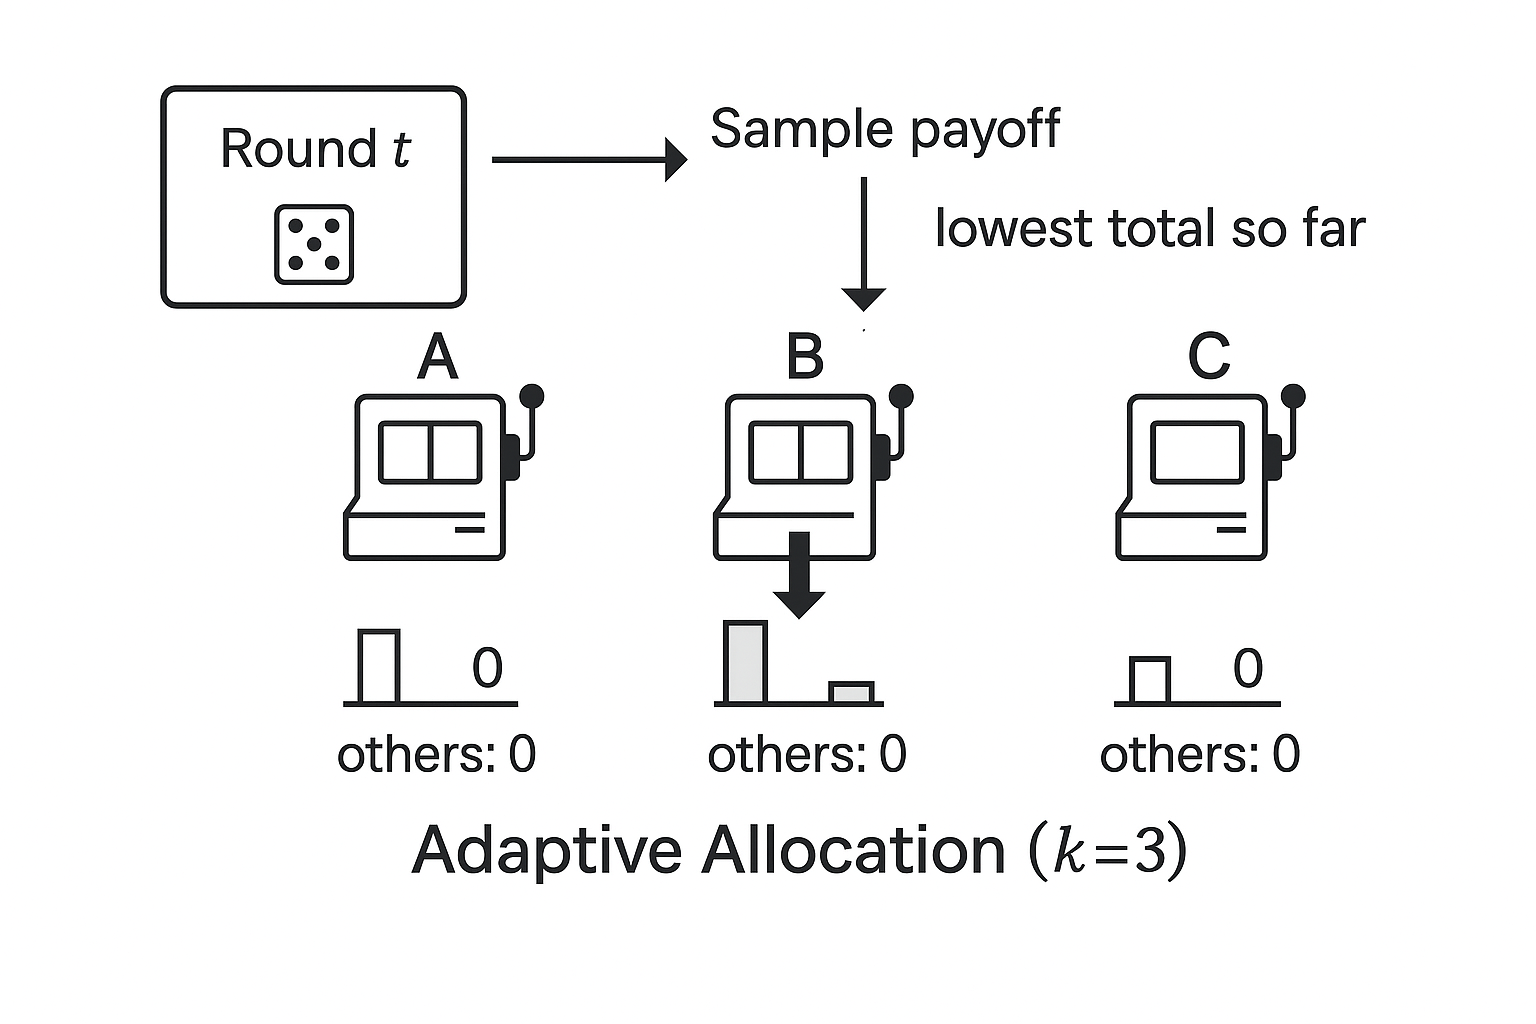
\includegraphics[width=0.45\textwidth]{../figures/Image_A.png}
\end{frame}

\begin{frame}{Part 1A: Results}
\begin{columns}[T,onlytextwidth]
  \column{0.5\textwidth}
  \centering
  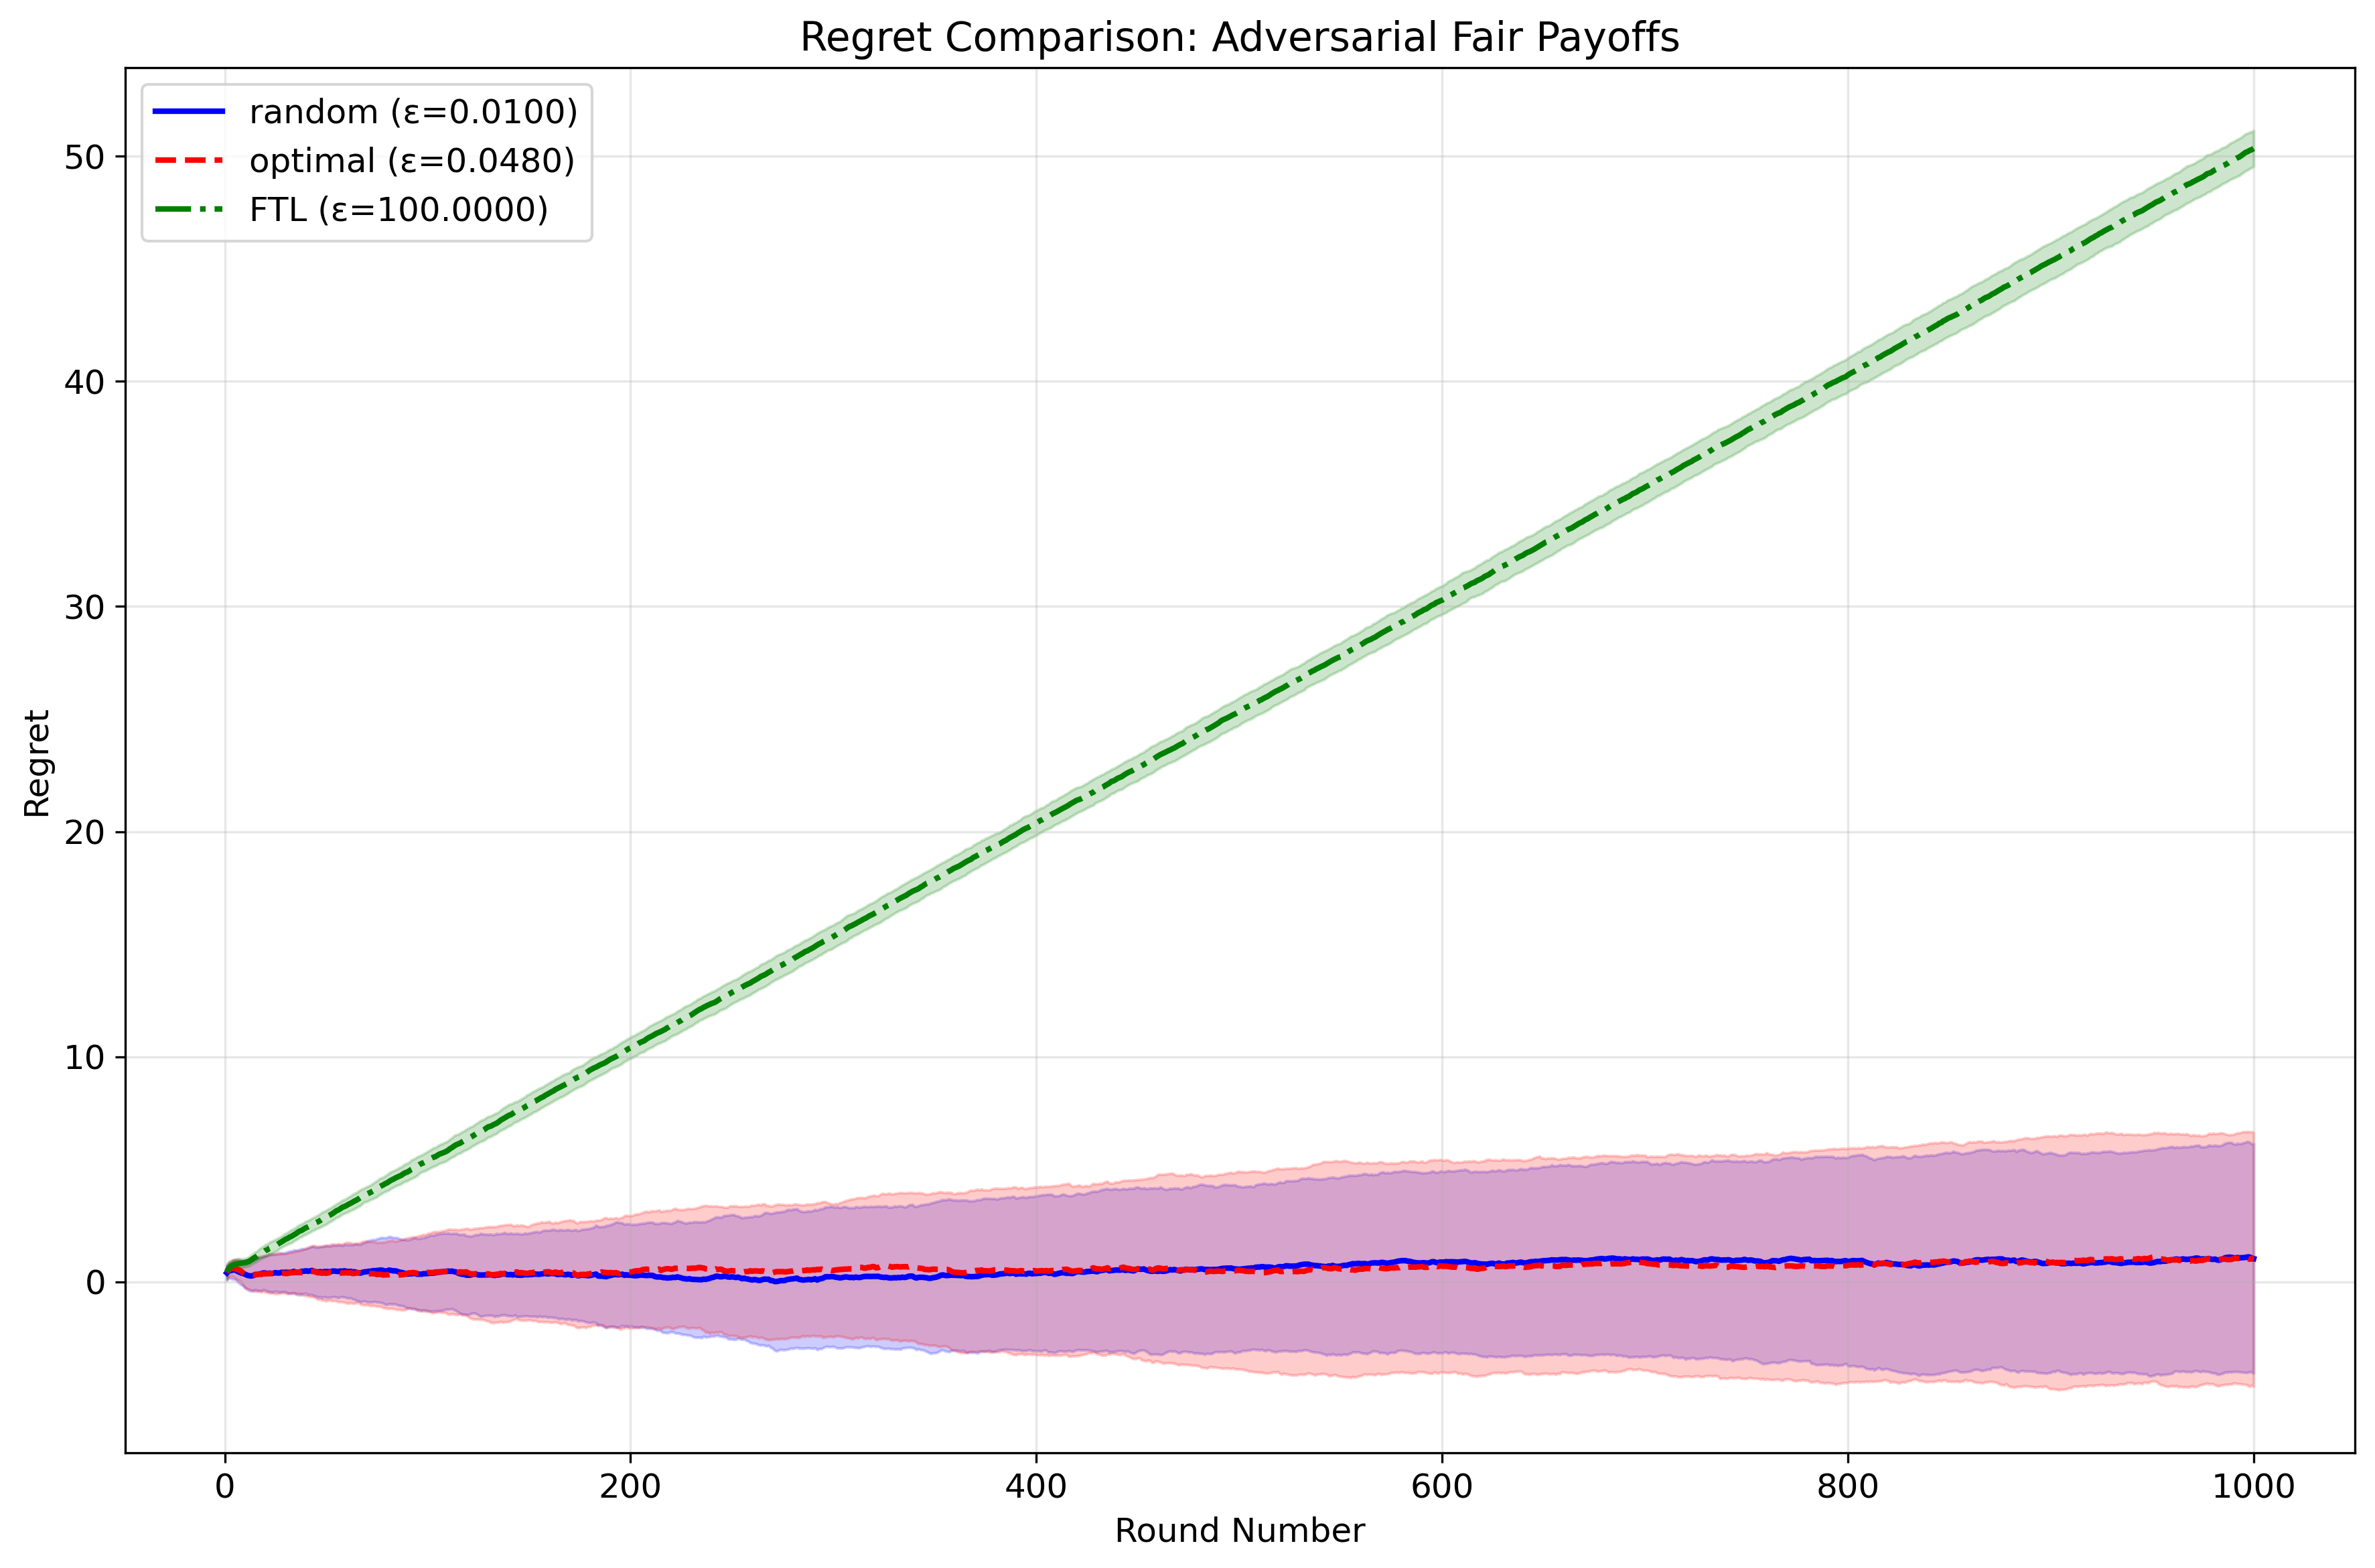
\includegraphics[width=\linewidth]{../figures/adversarial_regret_comparison.png}

  \column{0.5\textwidth}
  \centering
  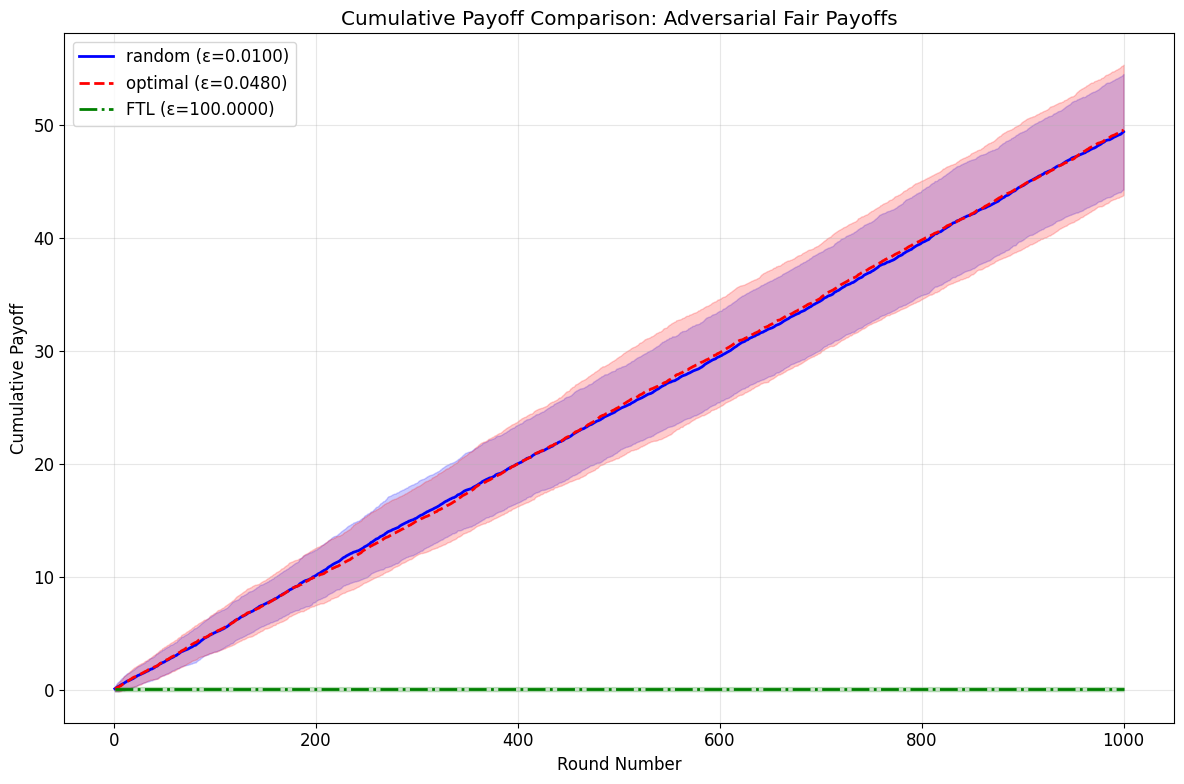
\includegraphics[width=\linewidth]{figures/AFR_payoff.png}
\end{columns}
\vspace{0.3em}
\small \textit{Note:} With $\epsilon=\sqrt{\ln k/n}$, the bound is $\approx 110$ for $h=1,k=3,n=1000$; observed regret stays below this.
\end{frame}

\subsection{B : BP}

\begin{frame}{Part 1B (BP): Setting \& Intuition}
\textbf{Setting}
\begin{itemize}
  \item Fix $p_j\in[0,1/2]$; each round $v_j^i\sim \mathrm{Bernoulli}(p_j)$; full information.
  \item $k=3$, $n=1000$.
\end{itemize}
\textbf{Intuition}
\begin{itemize}
  \item Stationary environment with a best arm $\Rightarrow$ FTL quickly locks in and achieves low regret.
  \item Random / theoretical $\epsilon$ explore more and lag.
\end{itemize}
\centering
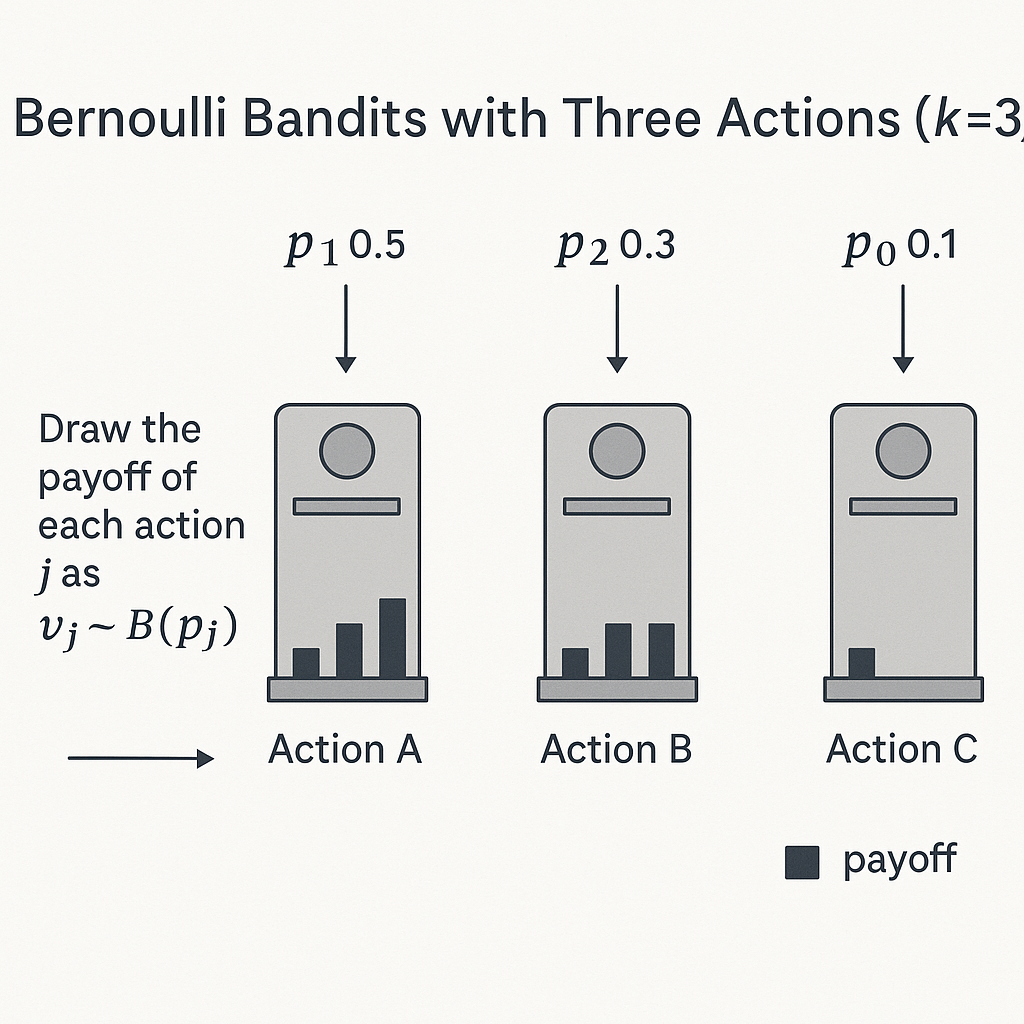
\includegraphics[width=0.4\textwidth]{../figures/Image_B.png}
\end{frame}

\begin{frame}{Part 1B: Results}
\begin{columns}[T,onlytextwidth]
  \column{0.5\textwidth}
  \centering
  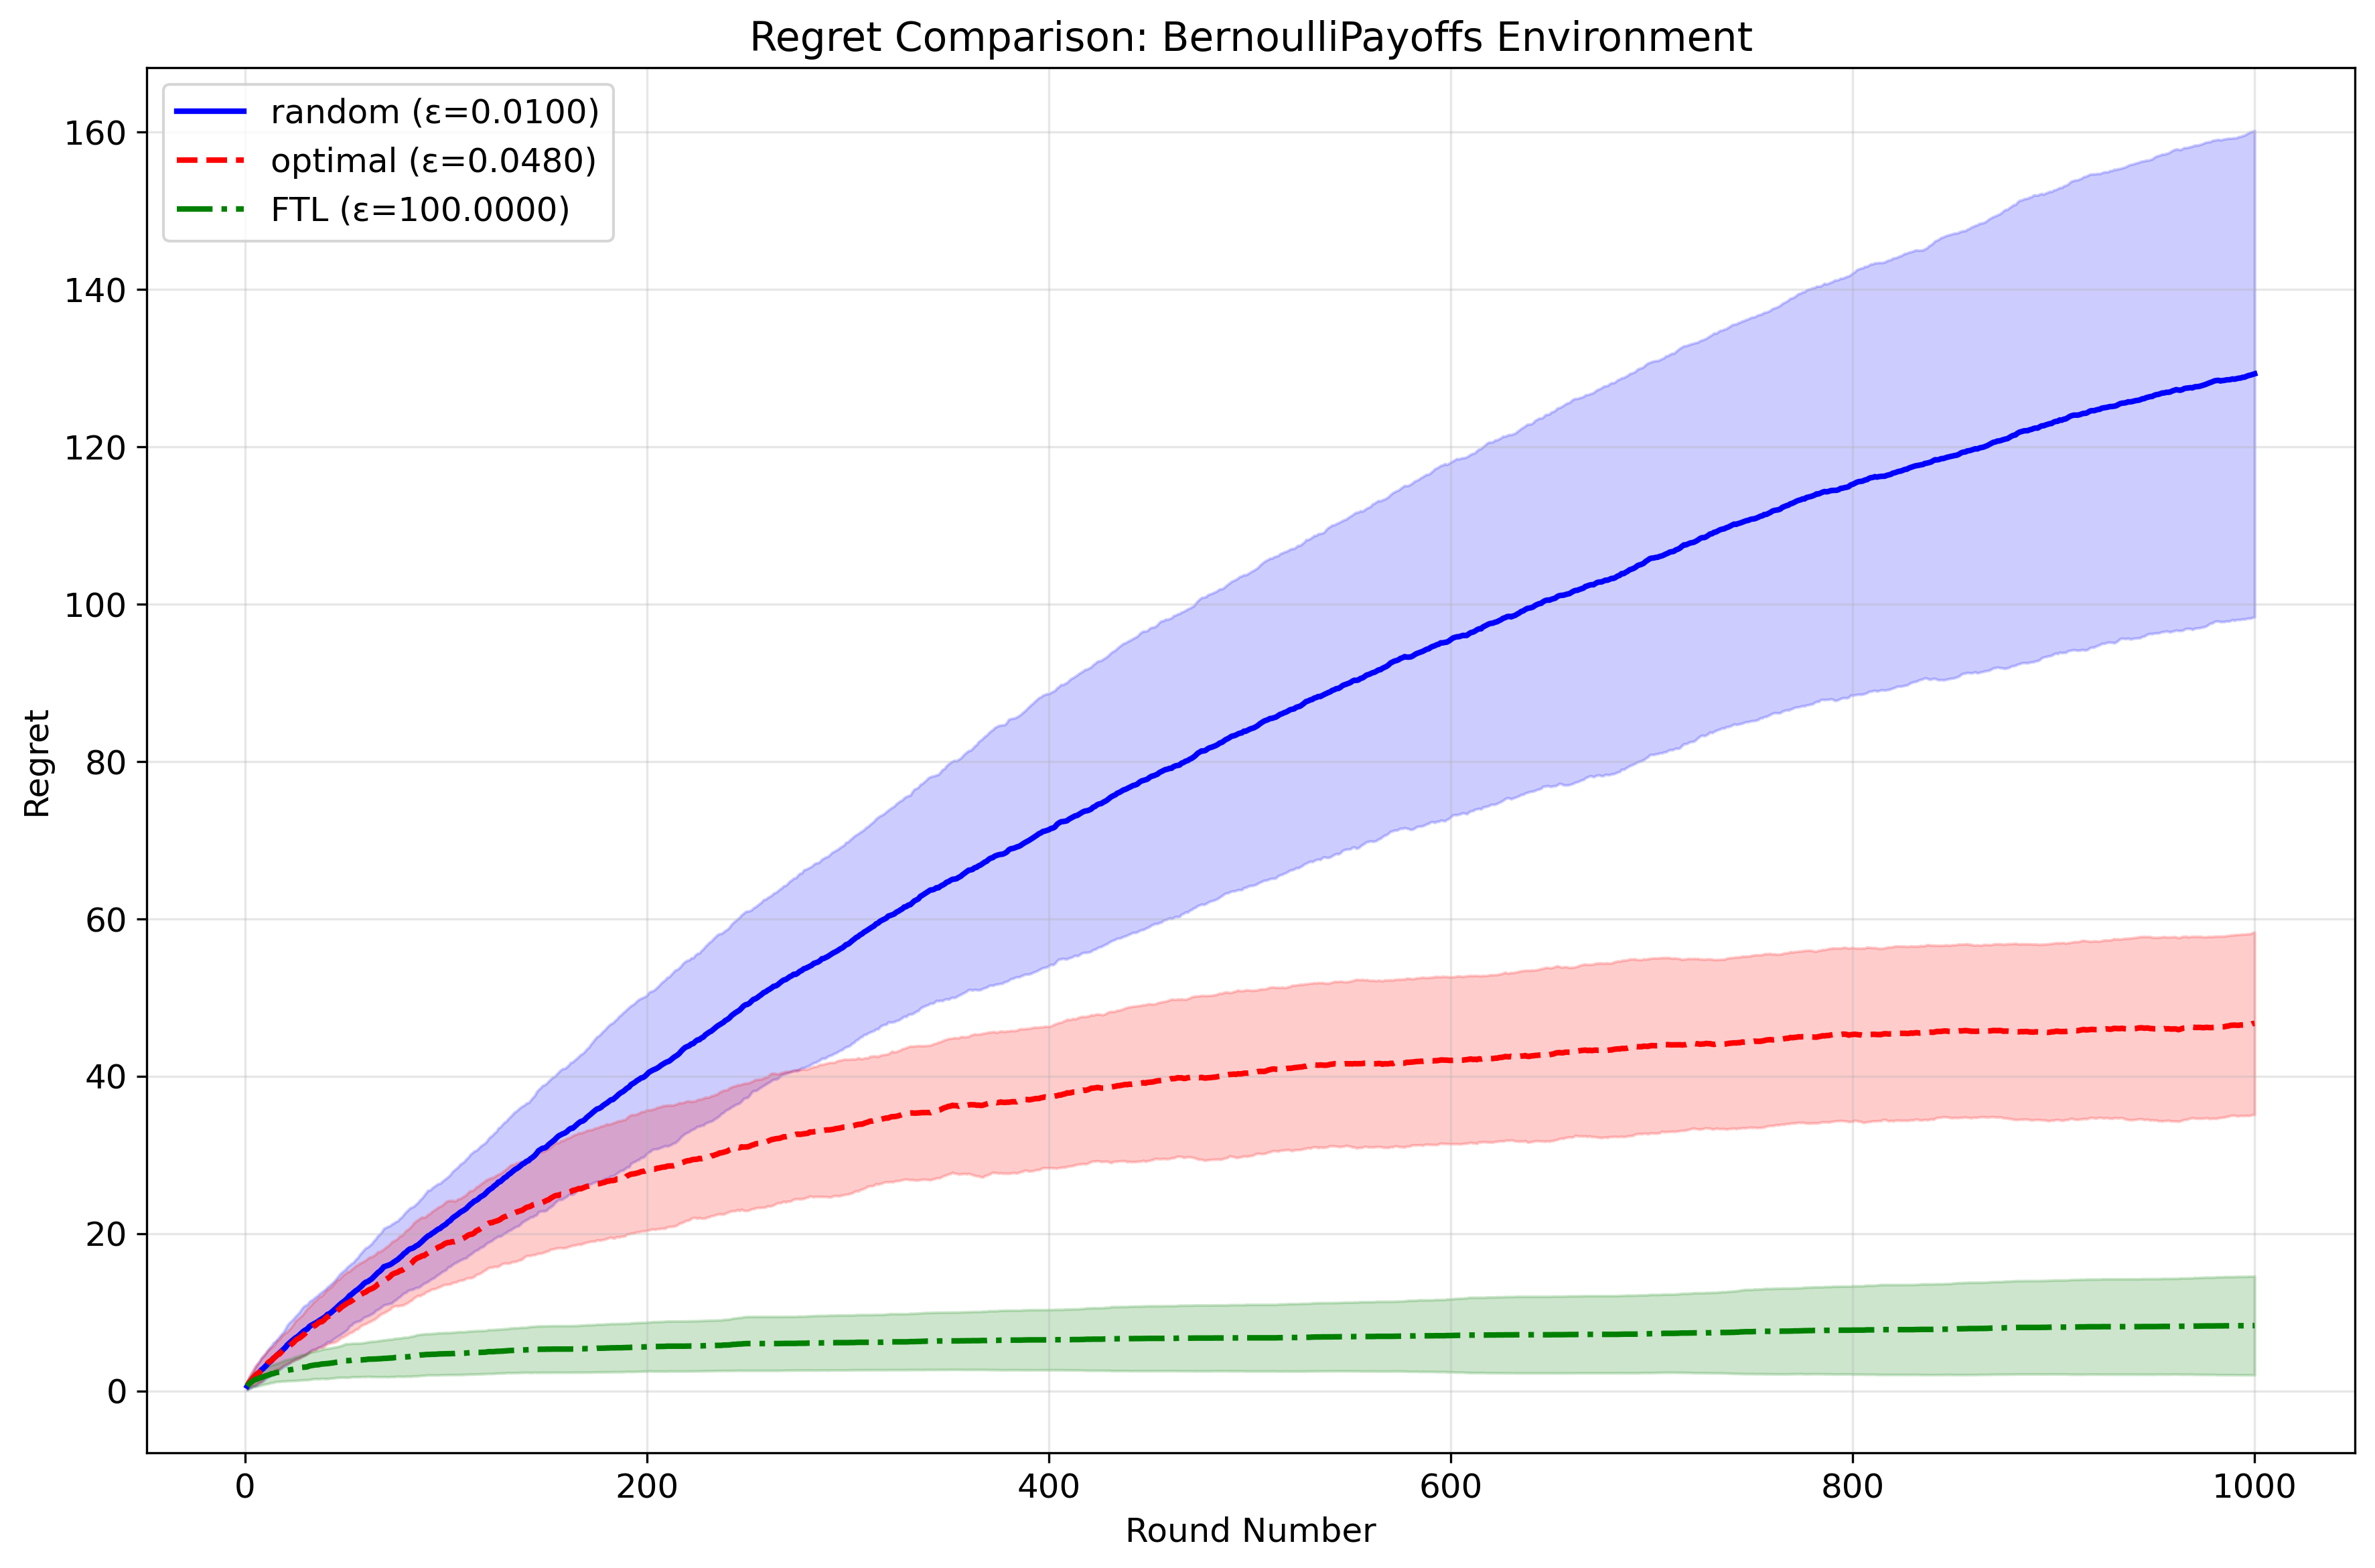
\includegraphics[width=\linewidth]{../figures/bernoulli_regret_comparison.png}

  \column{0.5\textwidth}
  \centering
  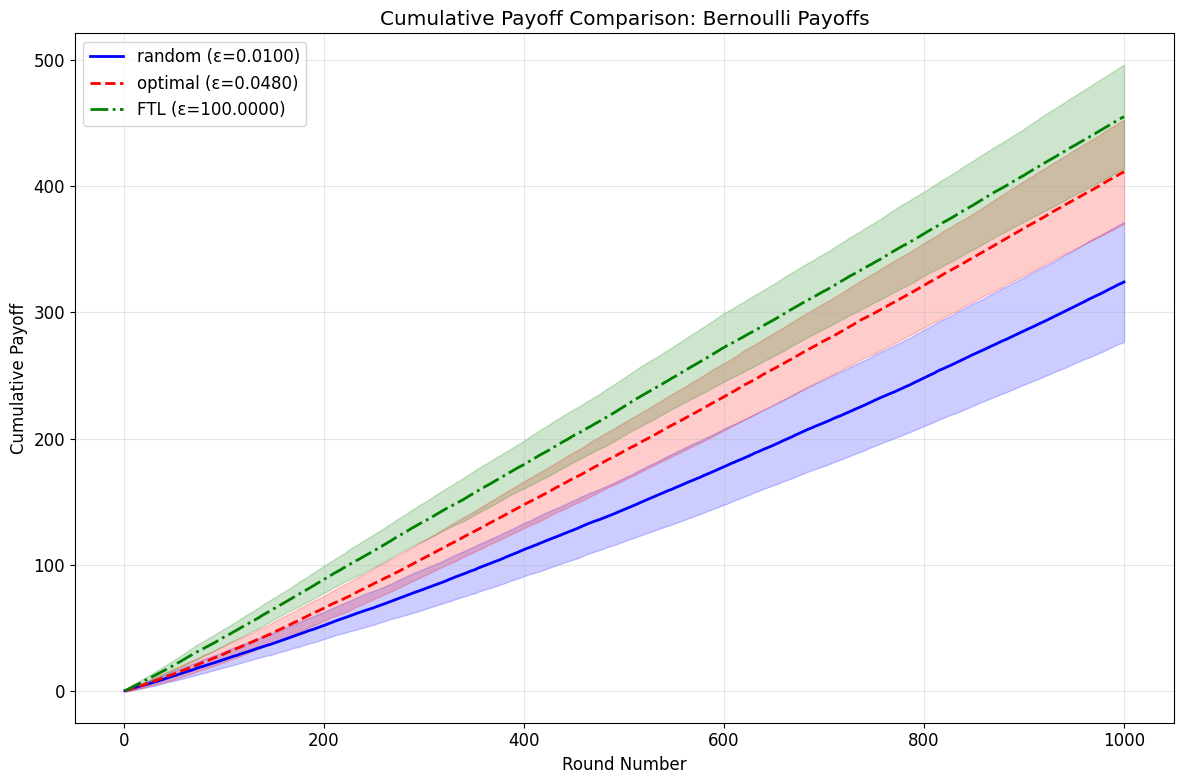
\includegraphics[width=\linewidth]{figures/BP_payoff.png}
\end{columns}
\vspace{0.3em}
\small \textit{Note:} Same theoretical ceiling applies; empirically FTL is best here.
\end{frame}

\section{Part 2}

% ---------- C (MERGED) ----------
\subsection{C : PP}

\begin{frame}{Part 2C (Pachinko): Methods, Data \& Intuition}
\textbf{Methods}
\begin{itemize}
  \item Treat each store as an arm; daily ROI normalized to $[0,1]$; full information.
  \item Five Tokyo stores; nonstationary ROI due to store setting changes.
\end{itemize}
\textbf{Intuition}
\begin{itemize}
  \item FTL (follow yesterday’s best store) works if ROI drifts slowly.
\end{itemize}
\centering
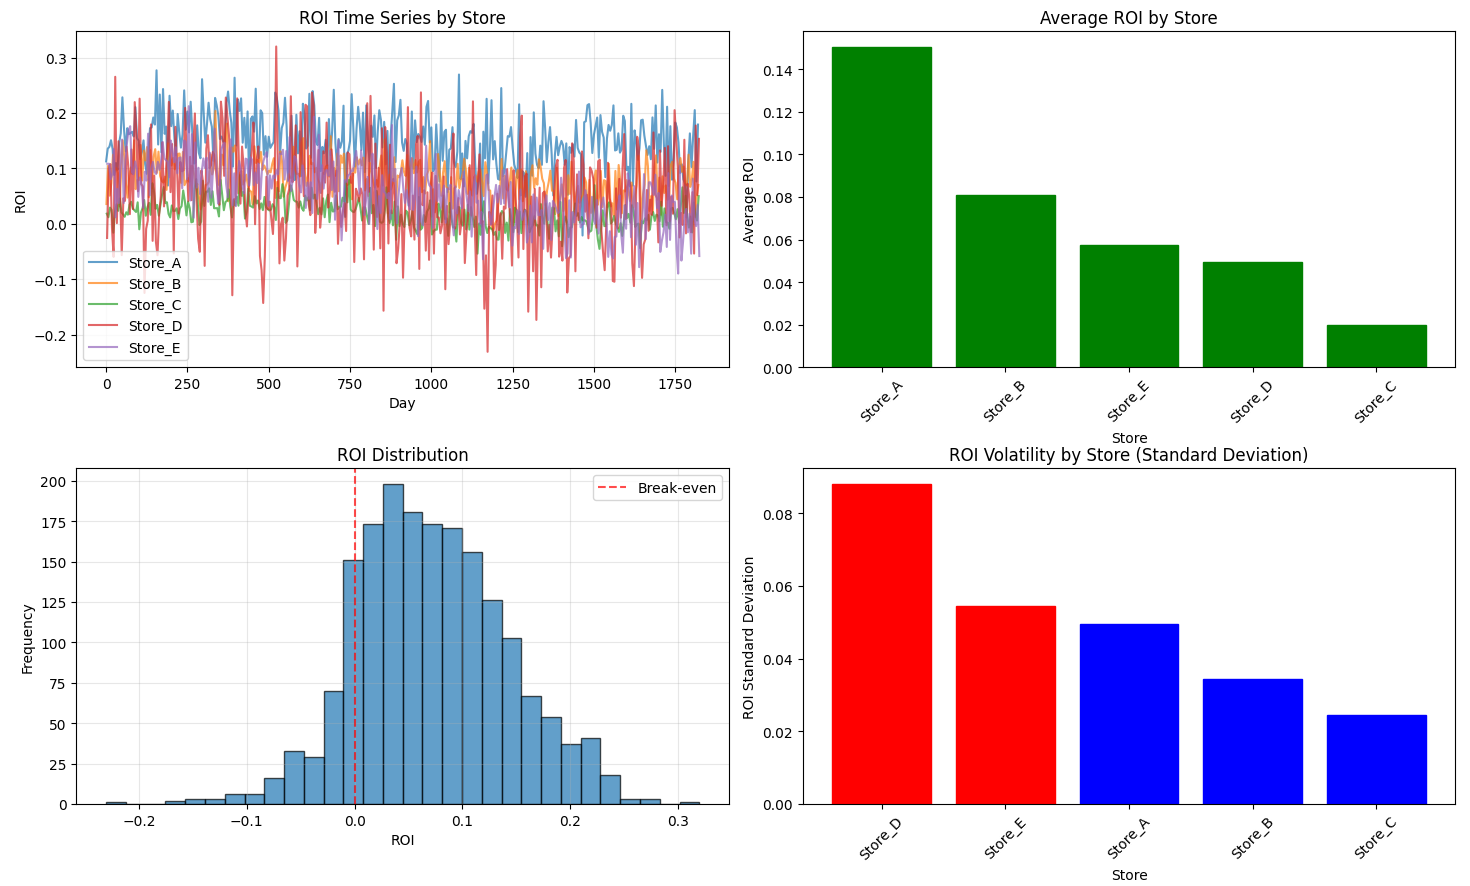
\includegraphics[width=0.72\textwidth]{332Project2/figures/ROI.png}
\end{frame}

\begin{frame}{Part 2C: Results}
\centering
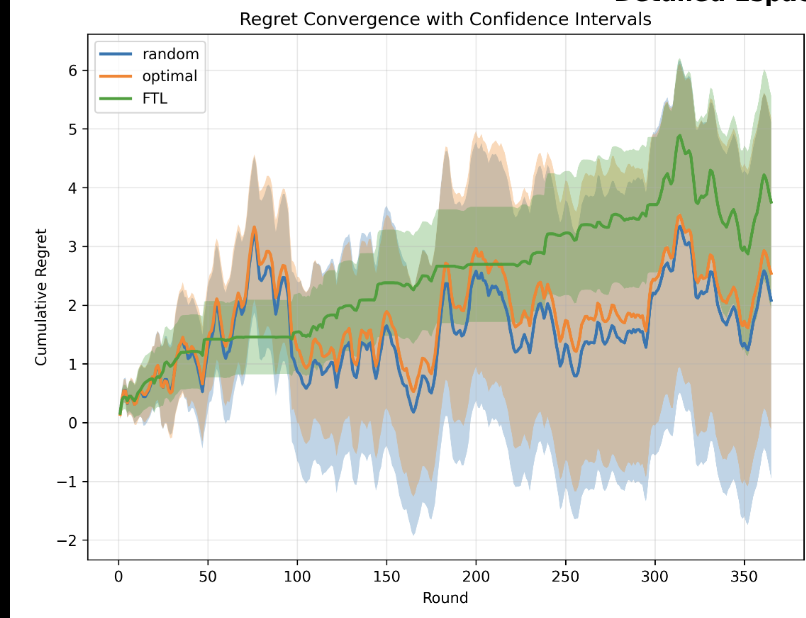
\includegraphics[width=0.6\textwidth]{332Project2/figures/Regret.png}\\
\small FTL regret $\to$ near zero; other rates underperform in this dataset.
\end{frame}

\subsection{D : RP}

\begin{frame}{Part 2D (RP): Model \& Algorithms}
\textbf{Model}
\begin{itemize}
  \item Clusters with intra-cluster correlation; hidden Markov regime selects a dominant cluster with persistence $p$.
  \item Agent allocates $w_t\in\Delta^N$; payoff $U_t=\alpha_t^\top w_t$.
\end{itemize}
\textbf{Algorithms}
\begin{itemize}
  \item FTL (past leader), Uniform (even split), EW/EG: $w_{t+1,i}\propto w_{t,i}e^{\varepsilon \alpha_{t,i}}$.
\end{itemize}
\textbf{Intuition} FTL overfits after switches; Uniform under-exploits; EW/EG balances adapt/exploit.
\end{frame}

\begin{frame}{Part 2D: Results \& Takeaways}
\begin{columns}[T,onlytextwidth]
  \column{0.5\textwidth}
  \centering
  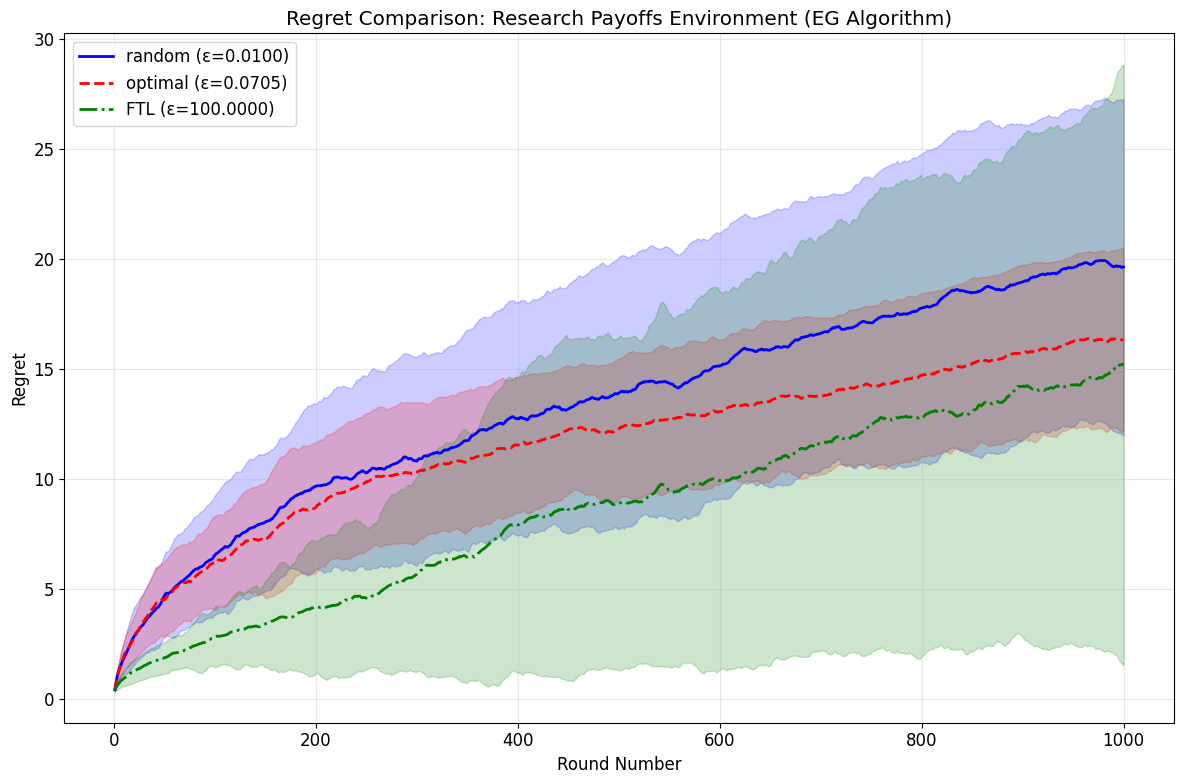
\includegraphics[width=\linewidth]{332Project2/figures/RP_regret.png}

  \column{0.5\textwidth}
  \centering
  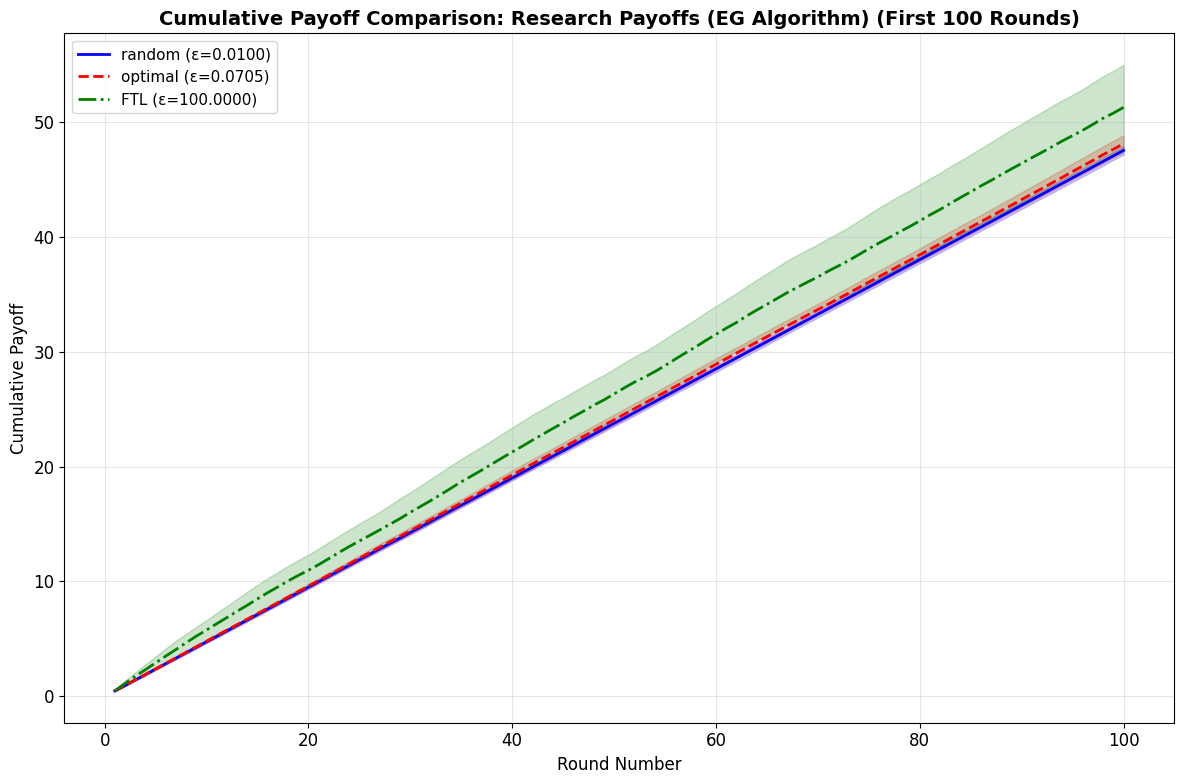
\includegraphics[width=\linewidth]{332Project2/figures/RP_payoff.png}
\end{columns}
\vspace{0.3em}
\small EW/EG (moderate $\varepsilon$) tracks regime changes and achieves the lowest regret and highest payoff. FTL and Uniform do not have vanishing regret here.
\end{frame}

\section{Reference and Usage of AI}

\begin{frame}{Reference and Usage of AI}
\begin{itemize}
    \item \textbf{Pachinko store data:} Daily store-level ``balls in/out'' statistics obtained from \emph{SloRepo} (\url{https://slorepo.com}). Data accessed on October 22, 2025 (America/Chicago).
    \item AI assistance was used for coding and figure generation; final verification, interpretation, and responsibility rest with the authors.
\end{itemize}
\end{frame}

\end{document}